\documentclass[class=article, crop=false]{standalone}

\usepackage{graphicx}	% Including figure files
\usepackage{amsmath}	% Advanced maths commands
\usepackage{amssymb}
\usepackage{natbib}

\newcommand{\fthin}{f_{\rm thin\,disk,\,recent}}
\newcommand{\tcools}{t_{10^5\,{\rm K}}}
\newcommand{\tacc}{t_{\rm acc}}
\newcommand{\Mdot}{\dot{M}}
\newcommand{\Rvir}{r_{\rm vir}}
\newcommand{\nH}{n_{\rm H}}
\newcommand{\Tvir}{T_{\rm vir}}
\newcommand{\msun}{{\rm M}_\odot}
\newcommand{\vvir}{v_{\rm vir}}
\newcommand{\Nsample}{17}
\newcommand{\Rcirc}[0]{r_{\rm circ}}
\newcommand{\vc}[0]{v_{\rm c}}
\newcommand{\mturb}[0]{\mathcal{M}_{\rm turb}}

\begin{document}

\section*{Appendix D: Notes on Individual Galaxies}

% M11D
\begin{figure*}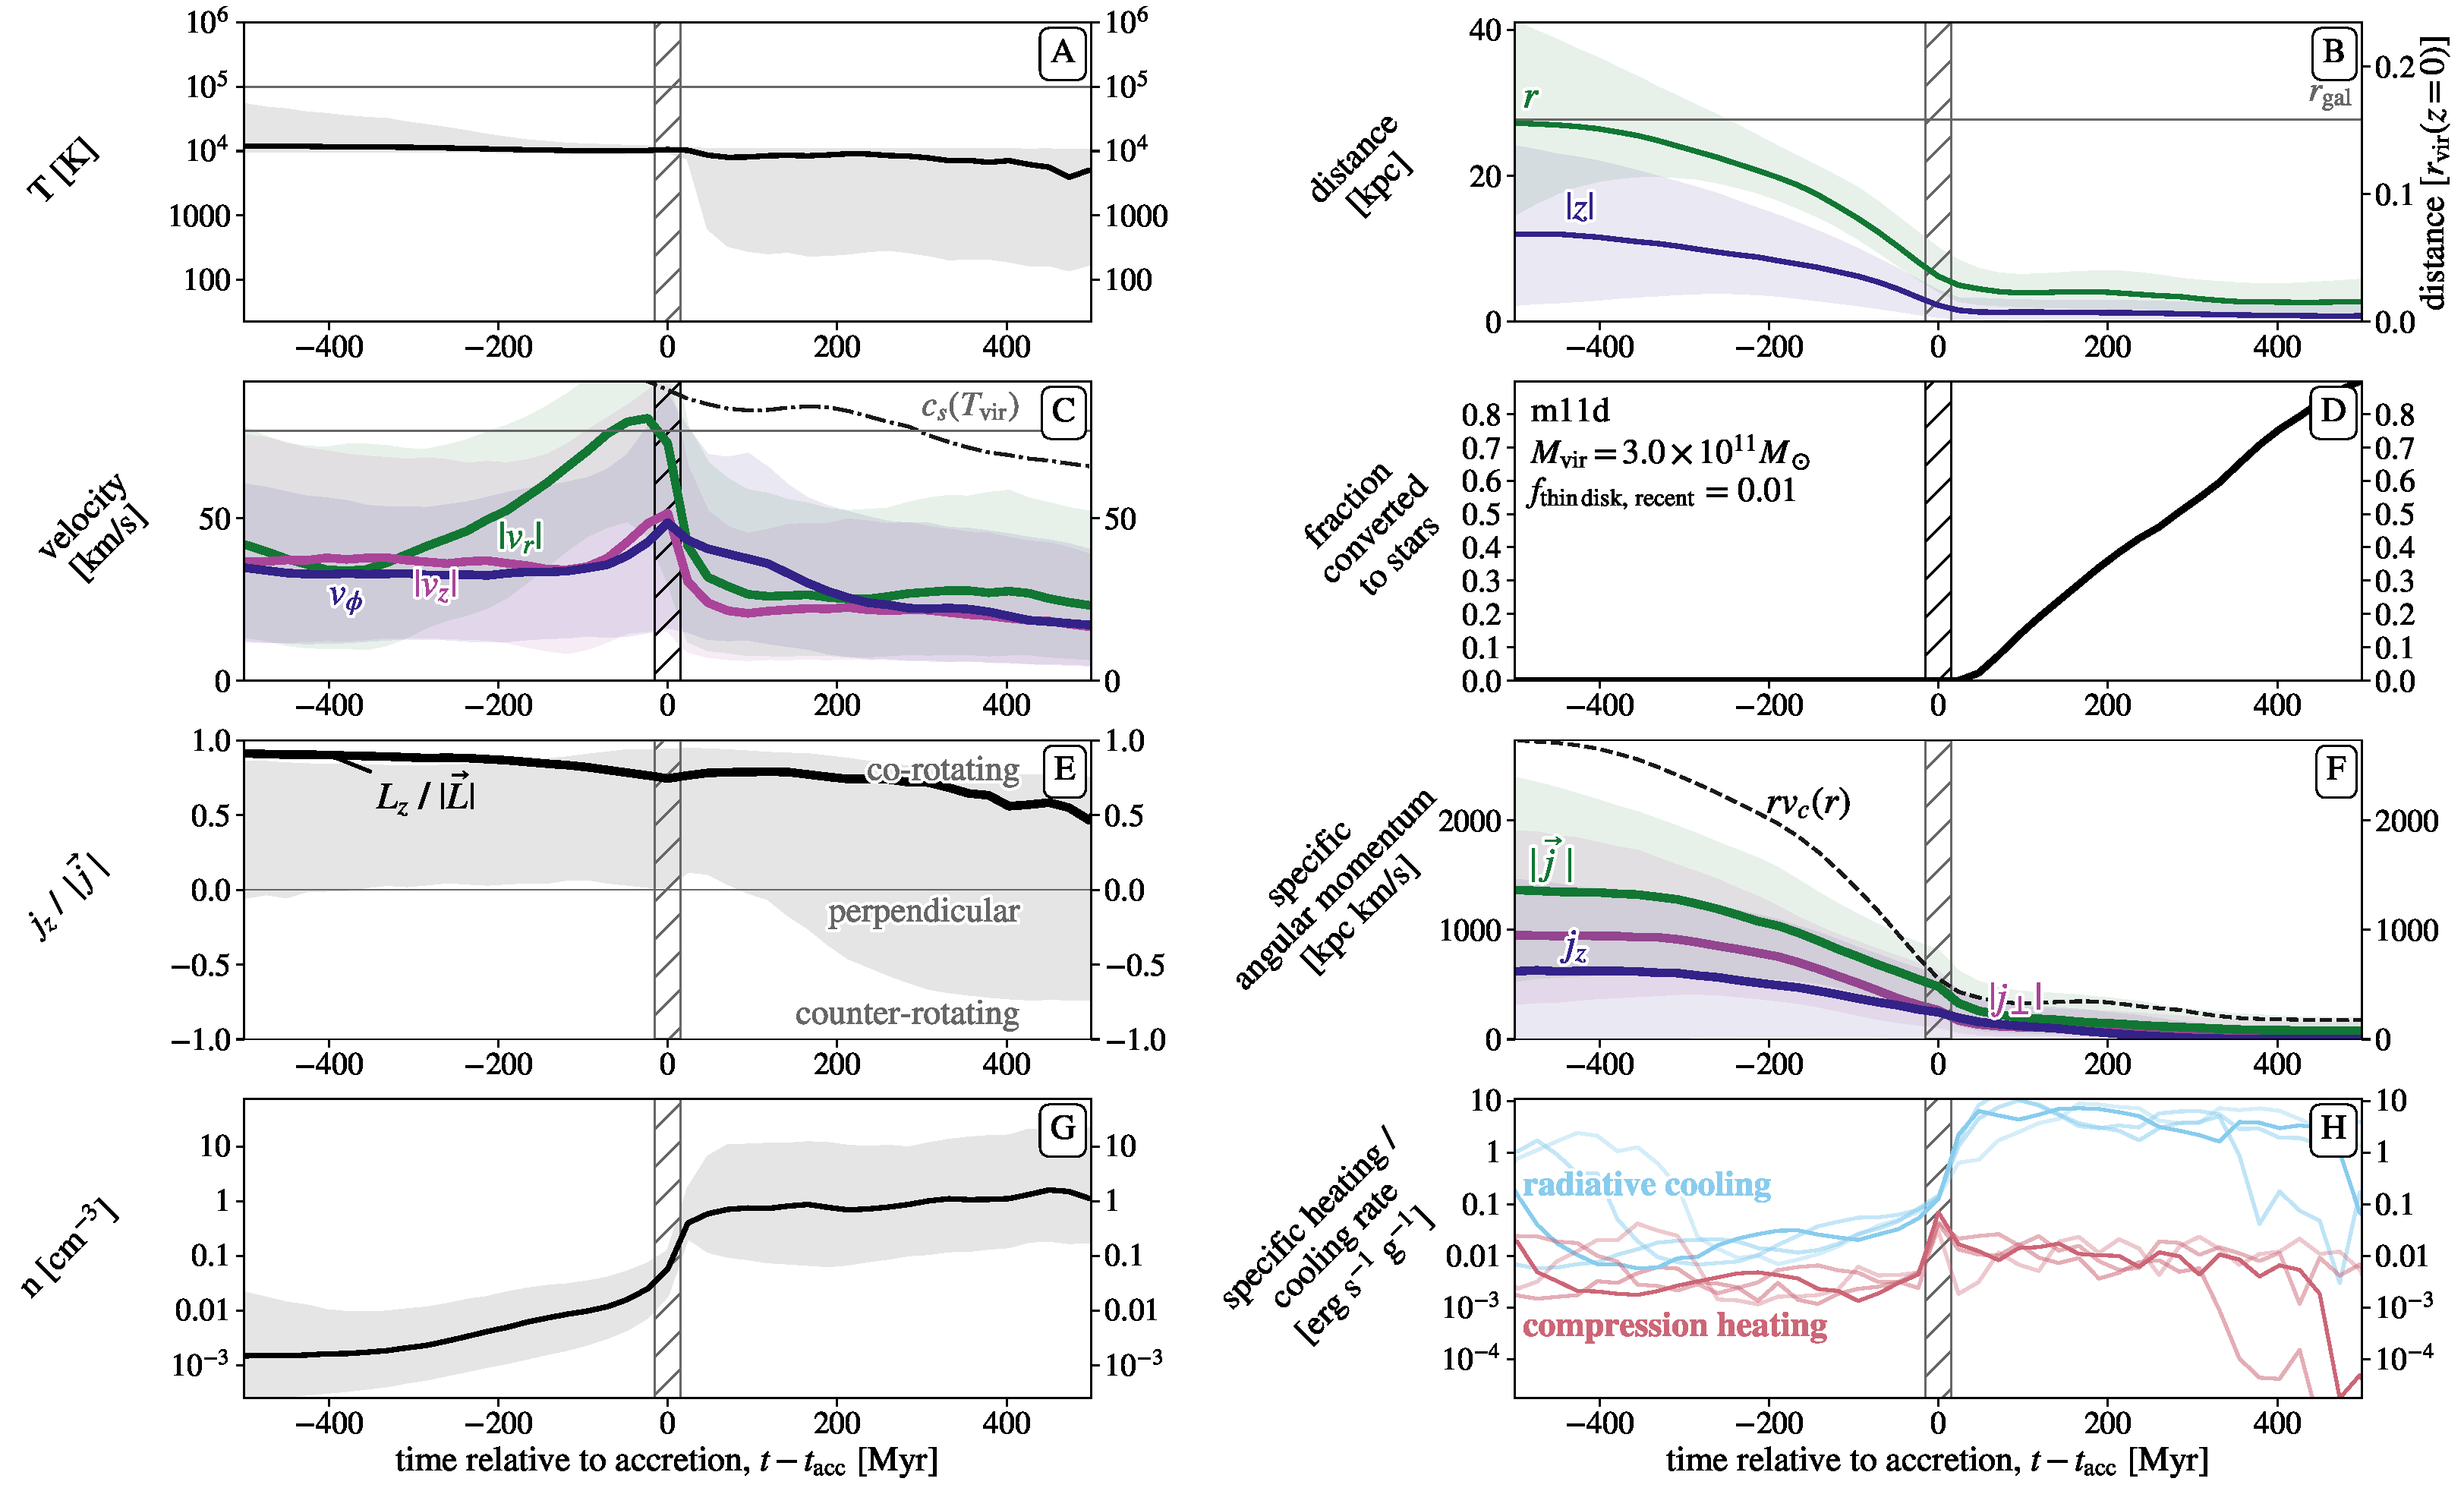
\includegraphics[width=\textwidth]{figures/variations/relative_to_accretion/before_and_after/before_and_after_allone_m11d_md.pdf}
\caption{
Temperature and geometry of gas accreting onto a $z\sim0$ galaxy in FIRE with a thin disk fraction $\fthin=0.03$ versus time relative to accretion ($t - \tacc$).
% This shows behavior for a single irregular galaxy, as a complement to Figs~\ref{f: before and after A},~\ref{f: before and after B}, and~\ref{f: before and after combined}.
In each panel solid lines and shaded regions mark the medians and 16th to 84th percentile ranges of all particles accreted within 1 Gyr prior to $z=0$.
\textbf{A:} Temperature.
\textbf{B:} 3D distance from halo center.
\textbf{C:} Velocity components of accretion (colored lines and band), relative to circular velocity at the median radius (dash-dotted line).
\textbf{D:} Fraction of gas converted into stars.
\textbf{E:} The ratio of $j_z / \vert \vec j \vert$, the cosine of the angle between the accreting gas and the galaxy angular momentum.
The dashed line shows this ratio for the total angular momentum of all accreted particles.
\textbf{F:} The magnitude of the specific angular momentum of particles ($\vert\vec{j}\vert$, green), the component of angular momentum aligned with the galaxy disk ($j_z$; purple), and the perpendicular component ($j_{\perp} = \vert \vec{j} - j_z \hat{z} \vert$; pink).
The dashed line shows the angular momentum necessary for rotational support.
\textbf{G:} Baryon number density.
\textbf{H:} Energy loss from radiative cooling (blue) and heating from $PdV$ work on the gas particles (red).
}
\label{f: m11d}
\end{figure*}

% M12F
\begin{figure*}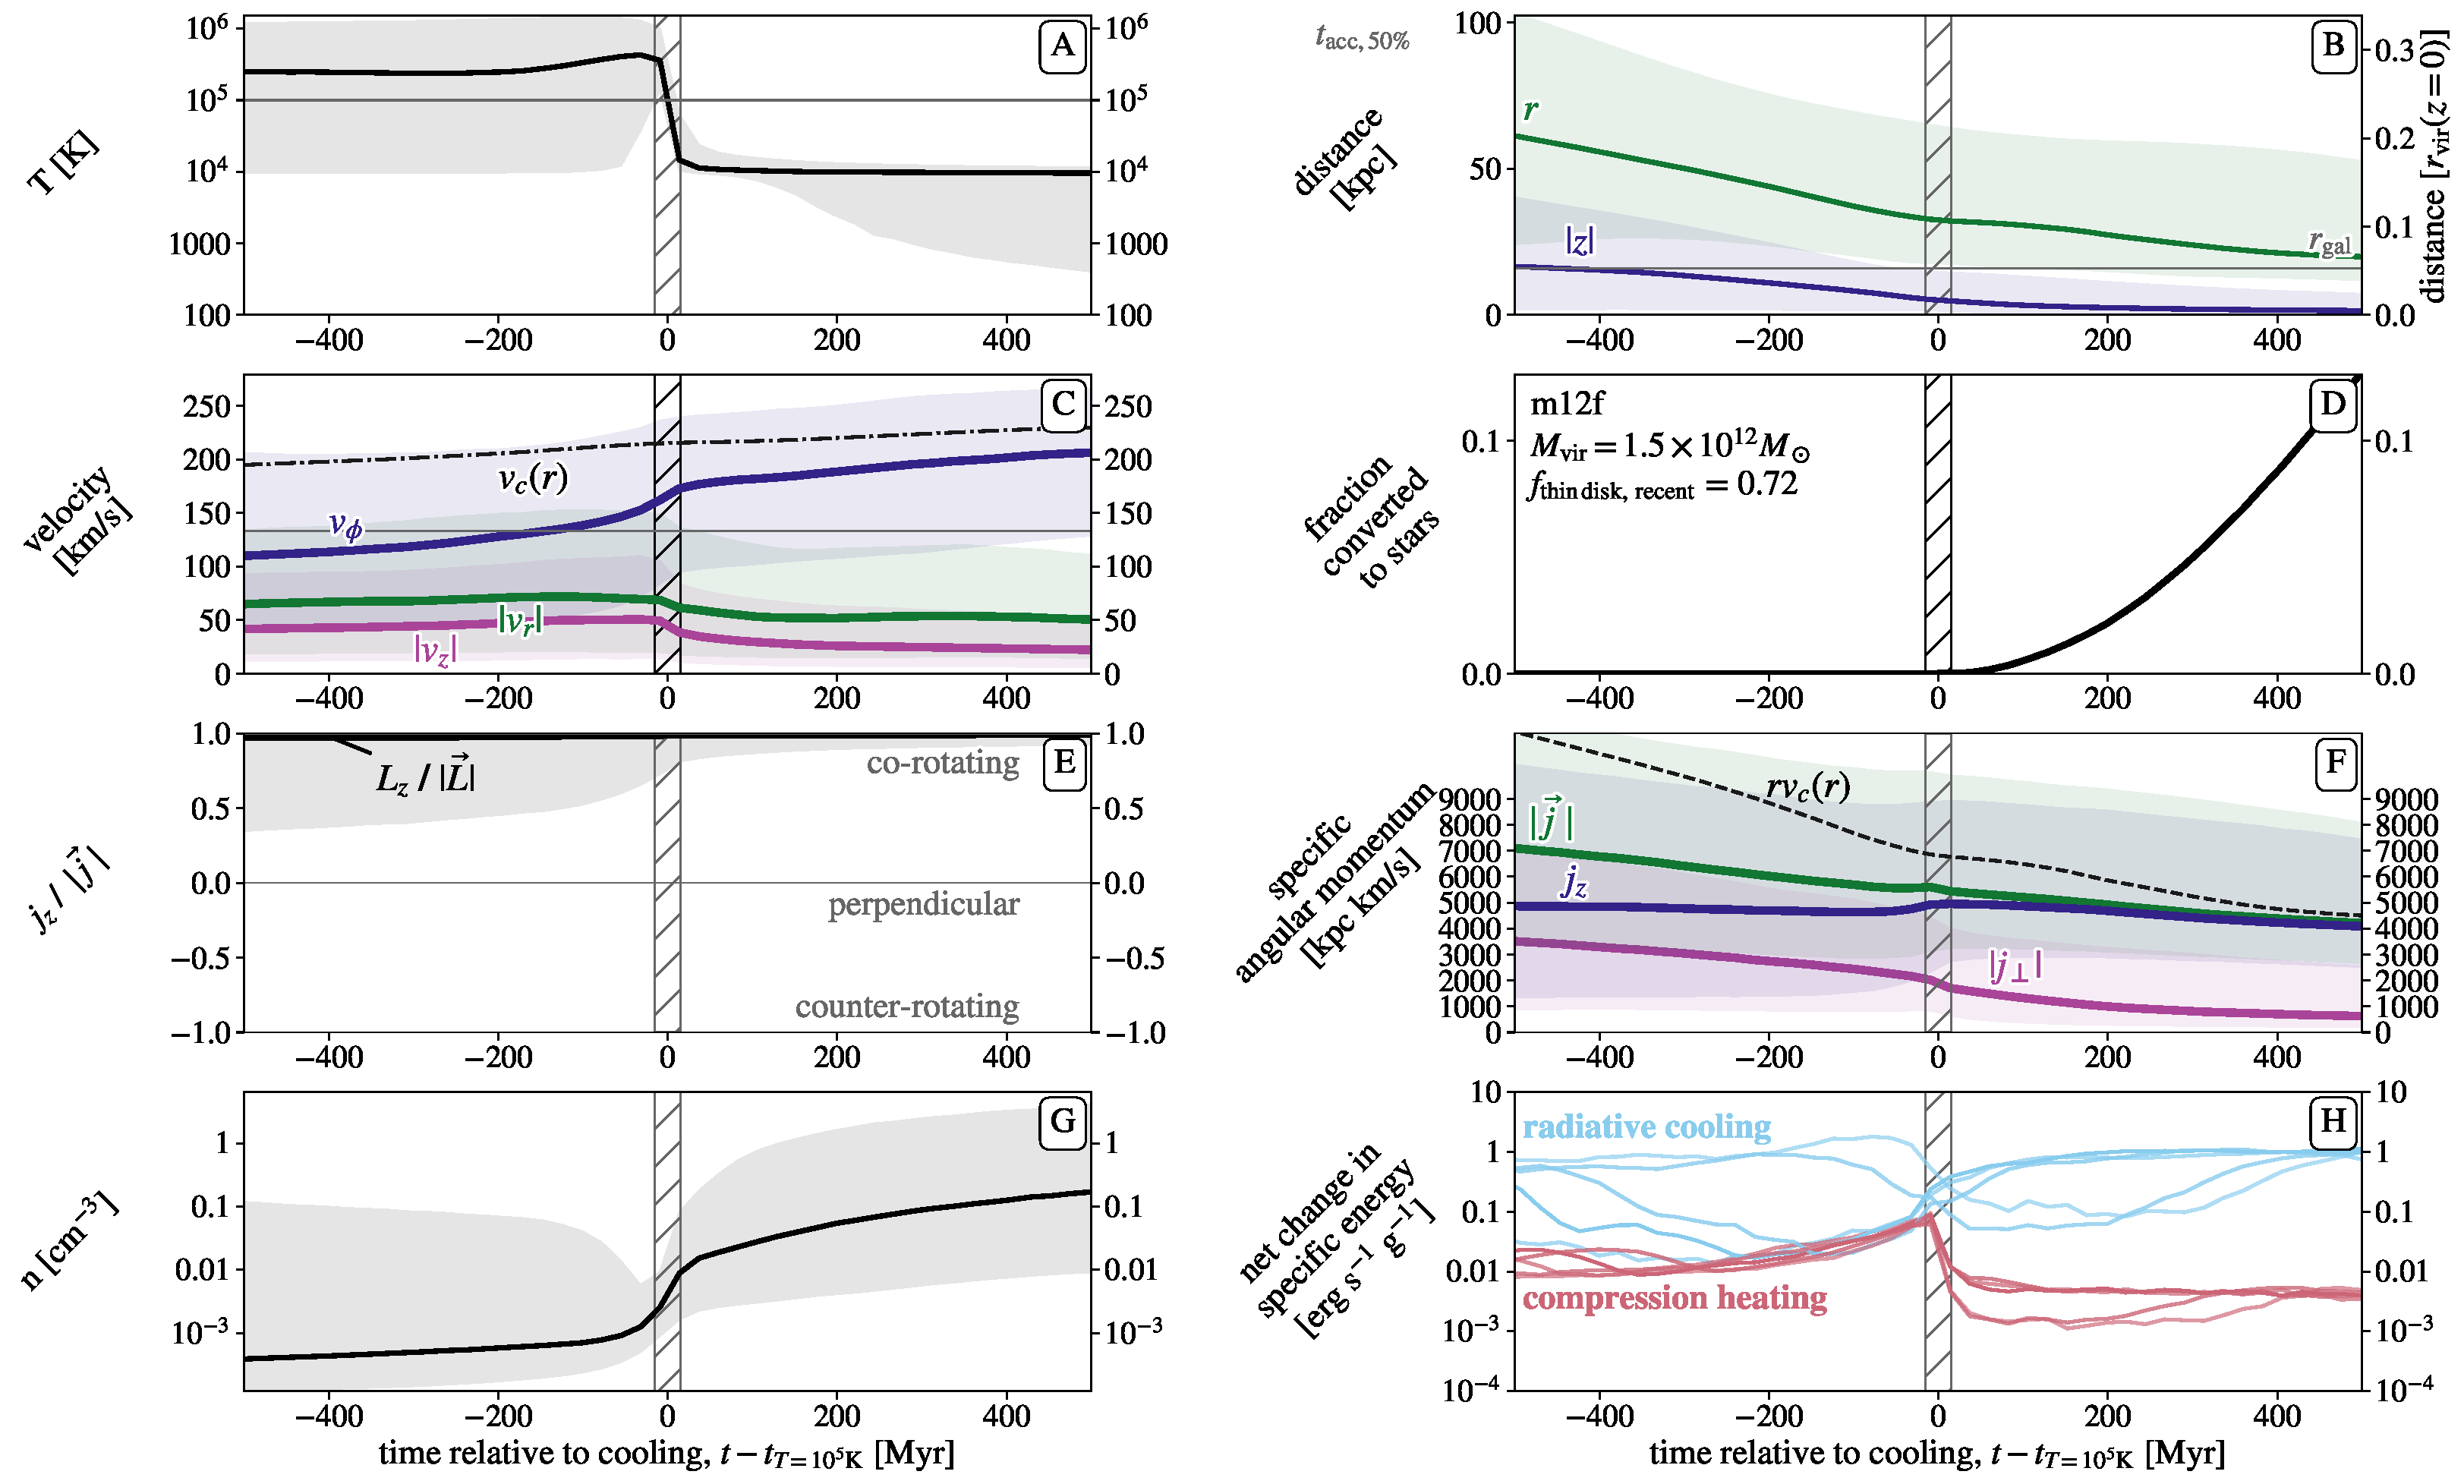
\includegraphics[width=\textwidth]{figures/before_and_after/before_and_after_allone_m12f_md.pdf}
\caption{
Same as Figure~\ref{f: m11d} but for accretion onto a $z\sim0$ galaxy in FIRE with a thin disk fraction $\fthin=0.87$ and versus time relative to the final cooling time ($t - \tcools$).
This galaxy (\texttt{m12f}) has qualitatively similar properties to other thin disk galaxies relative to $t-\tcools$, as seen via comparison with Figs~3,~6, and~7 in the main text.
}
\label{f: m12f-tcools}
\end{figure*}

% M12F
\begin{figure*}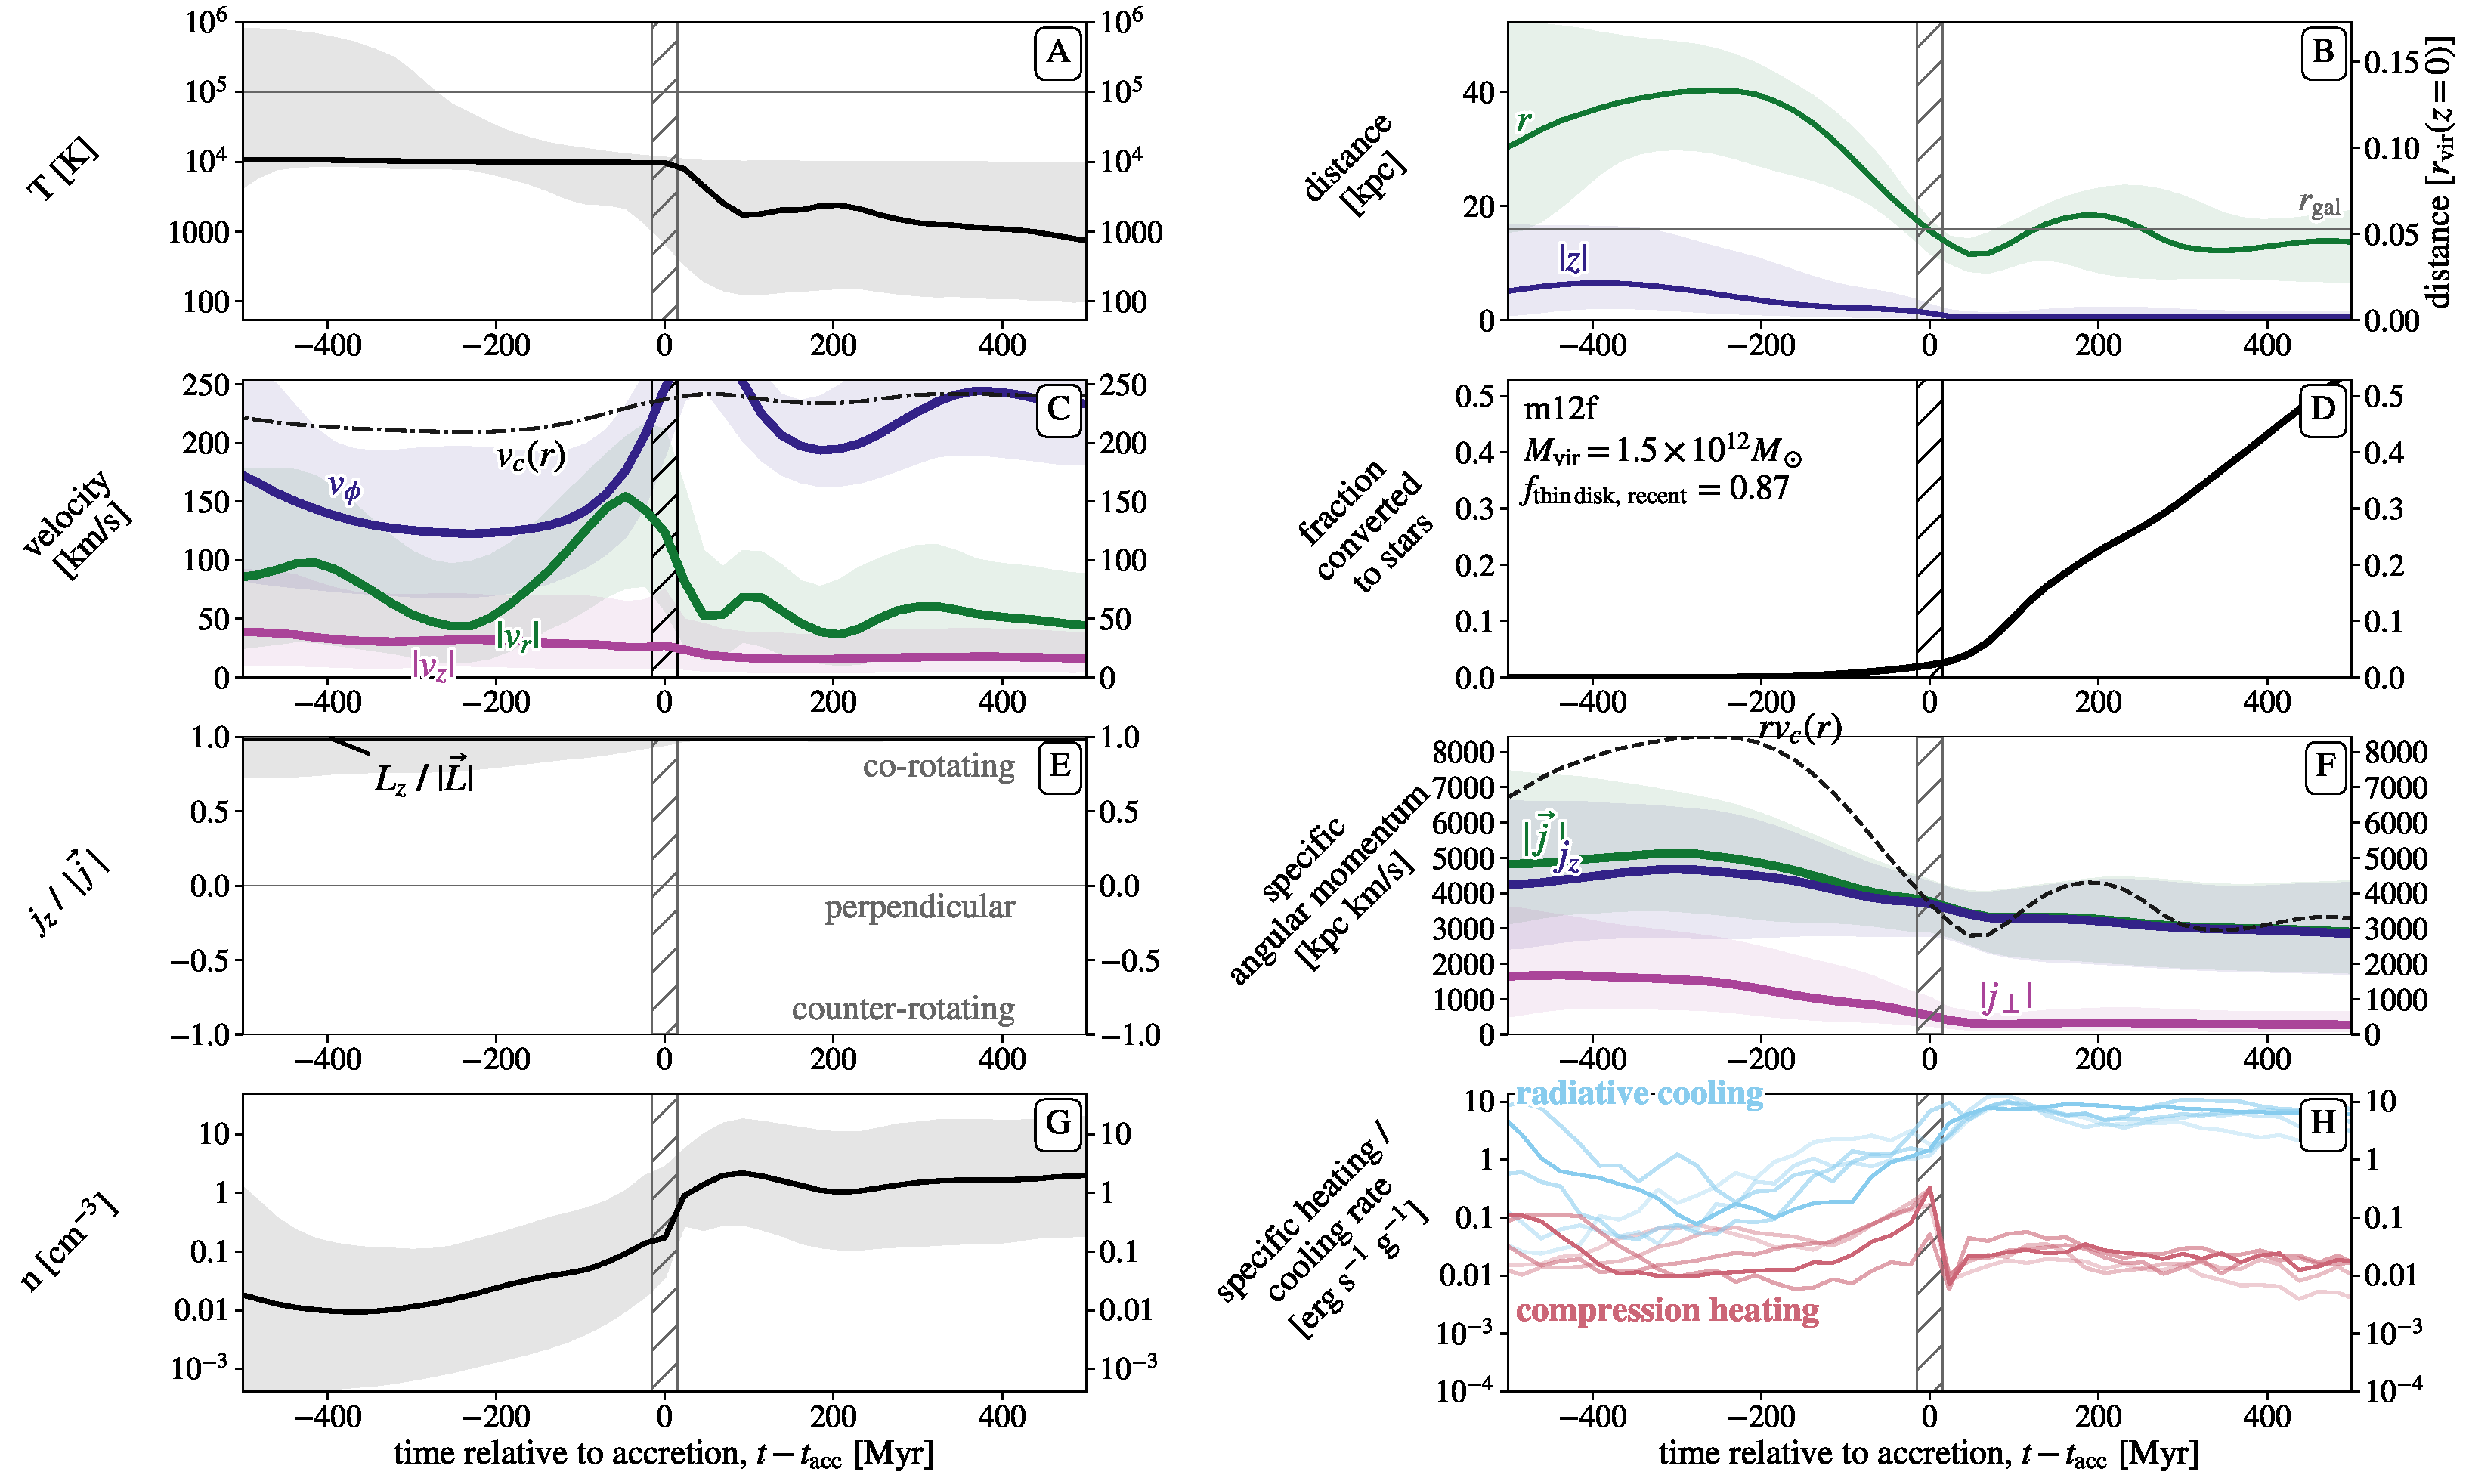
\includegraphics[width=\textwidth]{figures/variations/relative_to_accretion/before_and_after/before_and_after_allone_m12f_md.pdf}
\caption{
Same as Fig.~\ref{f: m12f-tcools}, but with time relative to $\tacc$ in the horizontal axis. 
In this galaxy the properties of accreting gas relative to $\tacc$ are qualitatively different from those relative to $\tcools$ shown in Fig.~\ref{f: m12f-tcools}, likely due to the relatively high specific angular momentum of the accreting gas (see text). 
% Gas circularizes and flattens at approximately twice the galaxy radius (Fig.~\ref{f: m12f-tcools}), and this figure shows that subsequently accretion onto \texttt{m12f} is already cooler and more aligned relative to other thin disk galaxies.
}
\label{f: m12f-tacc}
\end{figure*}

% M11D
In Figure~\ref{f: m11d} we show the equivalent of Figs~3 and~6 in the main text for a representative irregular galaxy, \texttt{m11d}.
Panel E shows that prior to $\tacc$ the accreting gas has a very broad and unchanging $j_z/\vert \vec j \vert$ distribution, in contrast with the narrowing angular momentum distribution of thin disk galaxies shown in the main text, and despite the total angular momentum being mostly aligned with the galaxy $(\Sigma \vec{j})_z / \vert \vec \Sigma\vec{j} \vert \sim 0.8-0.9$.
The low thin disk fraction of $0.03$ in this galaxy is thus  consistent with angular momentum coherence in accreted gas being necessary for thin disk formation. Other properties of the accretion onto m11d are apparent also in the sample average onto irregular galaxies (Fig.~7 in the main text) and are discussed there.

% M12F
Figures~\ref{f: m12f-tcools} and~\ref{f: m12f-tacc} show properties of accretion onto \texttt{m12f} (which was excluded from the averages in Fig.~7 in the main text) relative to $\tcools$ and $\tacc$ respectively.
Figure~\ref{f: m12f-tcools} shows that relative to $\tcools$ the accreting gas has the same key characteristics as accretion onto other thin disk galaxies --- inflow is hot in the CGM, and cooling is simultaneous with flattening, occuring when angular momentum support becomes significant.
Also, panels E and H show that angular momentum coherence increases prior to cooling, while radiative cooling in the hot gas is offset by compression heating.
By comparison, Fig.~\ref{f: m12f-tacc} shows that relative to $\tacc$ many of the properties of \texttt{m12f} are qualitatively different from those relative to $\tcools$, in contrast with other thin disk galaxies.
We suspect this difference is due to the relatively large specific angular momentum of accreted gas, which implies that the radius at which the accretion circularizes and cools is substantially larger than the galaxy radius, $\Rcirc \approx 2 r_{\rm gal}$ (see panel B in Fig.~\ref{f: m12f-tcools}).
As a result, gas reaches $r_{\rm gal}$ from within the disk, and quantities measured versus $\tacc$ track the evolution of gas accretion within the disk, rather than the evolution of accretion in the CGM. 

% Presence of a rotating cooling flow for intermediate cases
We also briefly discuss noticeable features of accretion onto additional specific galaxies.
The haloes with intermediate thin disk fractions $(0.1 \lesssim$ \\ $\fthin$ $< 0.6)$ also have intermediate levels of change in accretion alignment upon cooling (Fig.~5 in the main text). 
Four of these six haloes, \texttt{m12z}, \texttt{m12r}, \texttt{m12w}, and \texttt{m12m}, have $M_{\rm vir} \sim 10^{12} M_\odot$.
\texttt{m12z} has a chaotic halo with a number of ongoing mergers.
\texttt{m12r} has some ongoing thin disk formation, but is undergoing a major merger during the last Gyr that dominates the accreting gas supply and disrupts the galaxy structure.
This merger is relatively well-aligned with the disk, with $f_{\rm aligned} \approx 0.3-0.4$, and the aligned mass fraction does not change significantly as the gas cools past $\tcools$.
\texttt{m12w} is a galaxy where its inner CGM is only just virializing at $z=0$~(Yu et al., 2021), and the majority of the gas accretes with angular momentum perpendicular to the galaxy angular momentum.
Of these four the one with the highest thin disk fraction, \texttt{m12m}, 
% is a galaxy that undergoes significant rotating cooling flow accretion, but does not have a high thin disk fraction.
% Visual inspection reveals that \texttt{m12m} 
has a prominent stellar bar.
\texttt{m12m} may be evidence that if rotating cooling flows are a condition for disk formation, they are a necessary-but-not-sufficient condition (\S\S4.1 in the main text).
\texttt{m12m} is one of the few MW-mass halo simulations that does not include metal diffusion, which may also play a role in its morphology.
% The other two halos with an intermediate thin disk fraction have $M_{\rm vir} \sim 10^{11} M_\odot$ haloes,  \texttt{m11h} and \texttt{m11b}. These galaxies are beginning to form disks despite their lower virial mass.
% Much of their accretion is still isotropic, but alignment increases mildly post-cooling.

% \section{Comparison to metrics of galaxy and halo spin}

% % PREVALENCE OF QUIET ACCRETION -- VS angular momentum PROPERTIES
% \begin{figure*}
%     \centering
%     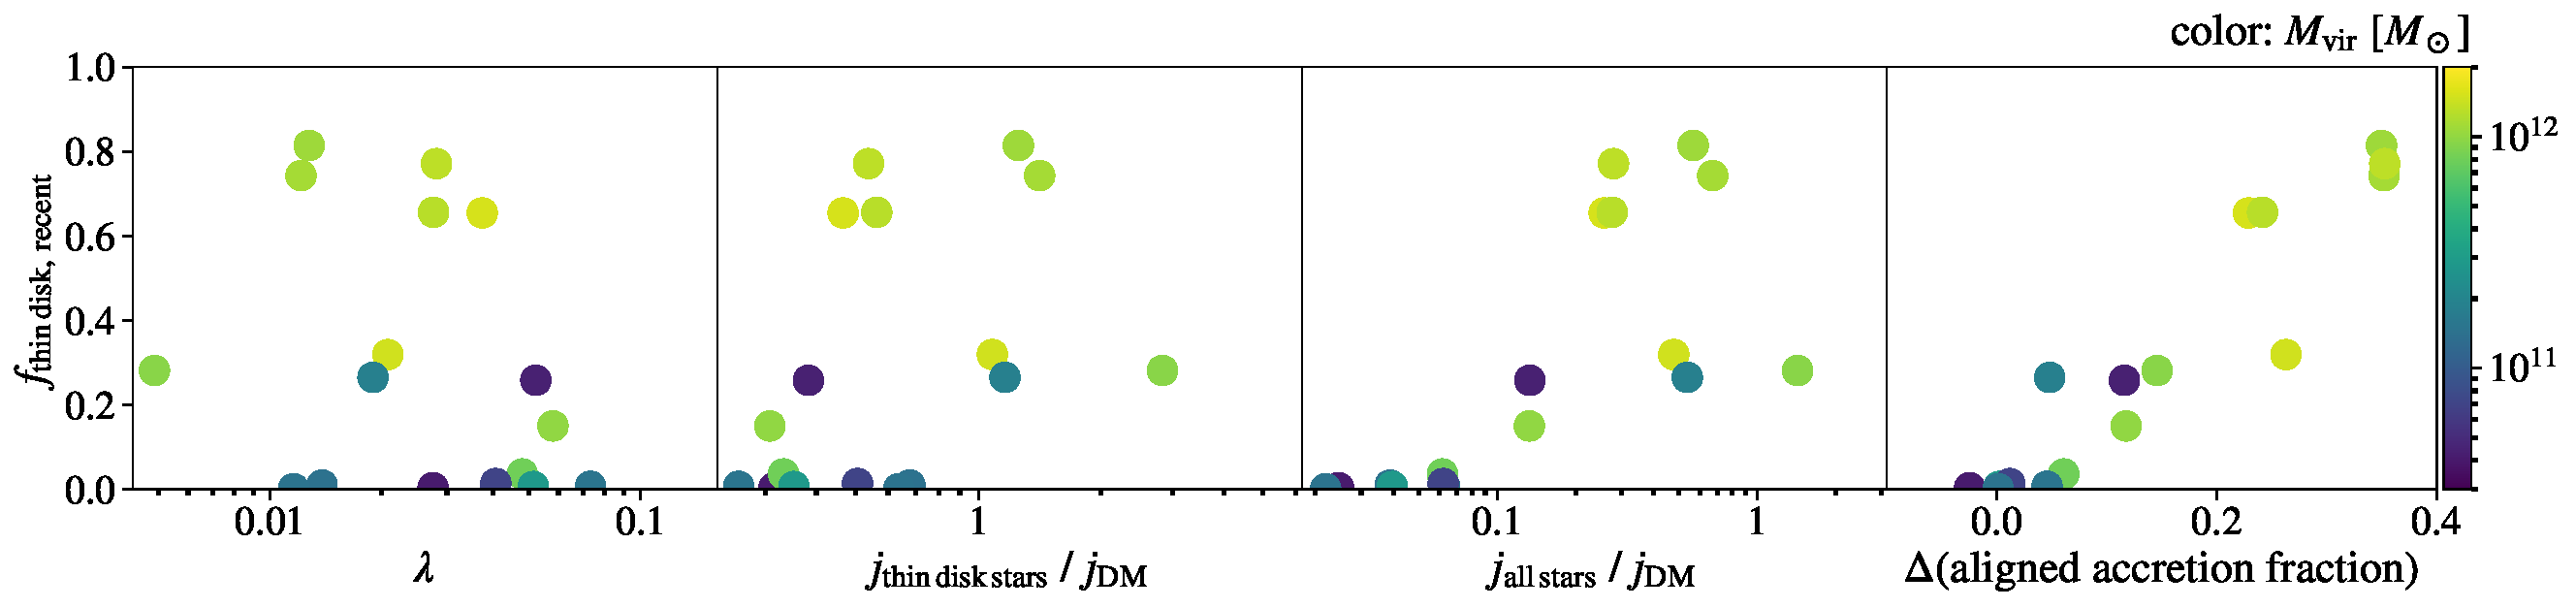
\includegraphics[width=\textwidth]{figures/prevalence/thin_disk_vs_angular_momentum_props.pdf}
%     \caption{
%     Fraction of young stars in a thin disk versus dark matter spin parameter $\lambda$, ratio of mean specific angular momentum of thin disk stars to that of the dark matter halo, ratio of mean specific angular momentum of all stars to that of the dark matter halo, and change in alignment of accreting gas (see Figure~\ref{f: prevalence}).
%     The last panel traces prevalence of rotating cooling flows, and correlates most strongly with thin disk fraction.
%     }
%     \label{f: prevalence vs j properties}
% \end{figure*}

% % Figure description
% Figure~\ref{f: prevalence vs j properties} compares the frequency of thin disks to some commonly used metrics of angular momentum properties.
% The left panel demonstrates there is no correlation between thin disk fraction and dark matter spin parameter, $\lambda \equiv j_{\rm DM} / ( \sqrt(2) r_{\rm vir} v_c(r_{\rm vir})$~\citep{Bullock2001} in our simulation sample, where $j_{\rm DM}$ is the magnitude of the total dark matter angular momentum within $r_{\rm vir}$, divided by the total dark matter mass.
% We also calculate $j_{\rm thin\,disk}$ ($j_{\rm all\,stars}$,  the magnitude of the total angular momentum of all thin disk stars in the galaxy, divided by the total mass of thin disk stars.
% Thin disk fraction and $j_{\rm thin\,disk} / j_{\rm DM}$ may be weakly correlated, but for the most part the thin disk stars in different galaxies have approximately the same specific angular momentum relative to $j_{\rm DM}$.
% Galaxies with a higher fraction of stars with $j_z / j_c(E) > 0.9$ often have a higher mean $j_{\rm all\,stars}$ than other galaxies with the $j_{\rm DM}$, as seen in the third panel.
% This may be in part because $j_c(E) \propto j_{\rm DM}$ for approximately constant $\lambda$ (both scale with dark matter mass) and $j_z \propto j$, therefore $j / j_{\rm DM} \sim j_z / j_c(E)$.
% The mean $j_{\rm all\,stars} / j_{\rm DM}$ of thin-disk galaxies is $\sim 0.3 - 0.7$ for all stars and $\sim 0.5 - 1$ for thin-disk stars, approximately consistent with observational constraints~\citep[e.g.][]{Fall2018, Posti2019}.
% Irregular galaxies have $j_{\rm all\,stars} / j_{\rm DM} \lesssim 0.1$, indicating that if accreting gas starts with approximately the same angular momentum as the dark matter then irregular galaxies must lose most of that angular momentum.
% The tracer of rotating cooling flow prevalence, shown in the rightmost panel, remains the strongest predictor of thin disk fraction.

\end{document}